This chapter presents the design and implementation of \bpfbox{}, an initial research
prototype of an \gls{ebpf}-based confinement framework. \bpfbox{} is the first
full-fledged confinement framework to leverage \gls{krsi}'s \gls{lsm} programs to enforce
high-level policy. Using \gls{ebpf}, it combines various behavioural aspects of the
sandboxed application from both userspace and kernelspace to enforce a simple, yet
fine-grained policy defined in a domain-specific policy language. This chapter was a part
of a previously published paper at CCSW'2020, co-authored with Anil Somayaji and David
Barrera~\cite{findlay2020_bpfbox}.



\section{\bpfbox{} Overview}

At a high level, \bpfbox{} is a confinement mechanism based on \gls{ebpf}. \todo{Outline basic components}

\todo{Describe how \bpfbox{} enforces policy from start to finish, refer to \Cref{fig:bpfbox-overview}}

\begin{figure}[htpb]
  \centering
  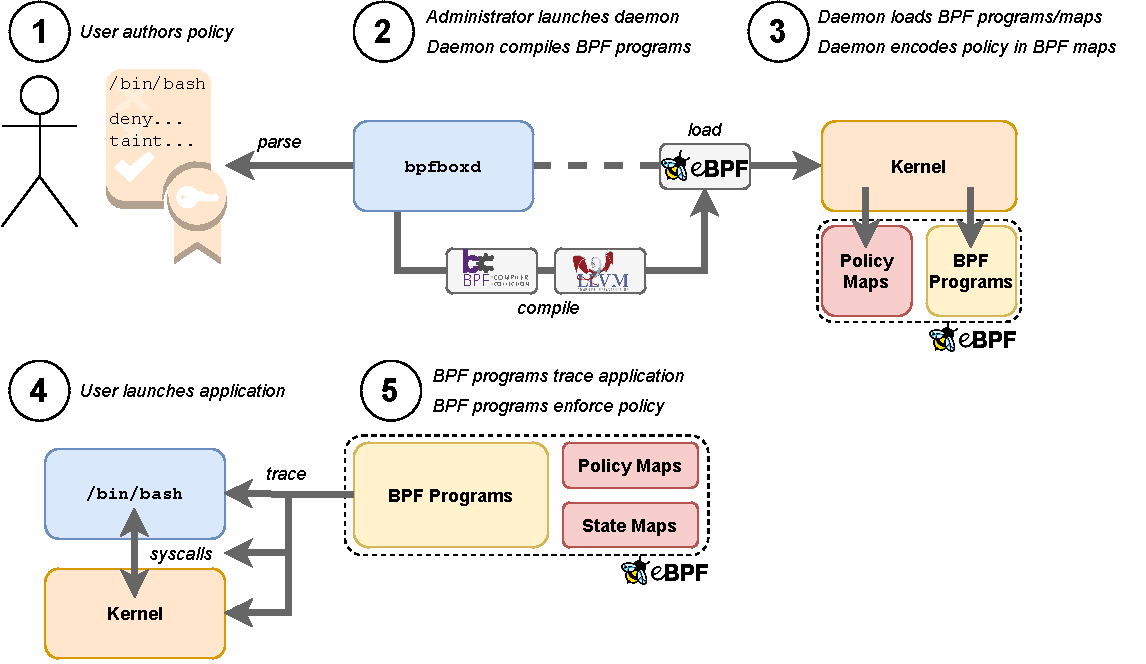
\includegraphics[width=0.8\linewidth]{figs/bpfbox/overview.pdf}
  \caption[A high-level overview of how \bpfbox{} confines applications]{
    A high-level overview of how \bpfbox{} confines applications. Users write policy files
    which the daemon encodes into \gls{ebpf} maps. The daemon loads these maps, along with
    policy enforcement and tracing programs into the kernel. At runtime, \bpfbox{}'s
    \gls{bpf} programs trace the application and enforce policy.
  }%
  \label{fig:bpfbox-overview}
\end{figure}

\bpfbox{}'s fundamental enforcement strategy is based on several \gls{bpf} program and map
types, summarized as follows. Maps are outlined in \textbf{\green{green}} and programs are
outlined in \textbf{\purple{purple}}. The reader is encouraged to revisit
\Cref{ss:bpf-programs-bg,ss:bpf-maps-bg} in \Cref{c:background}, where necessary, for
clarification on specific program and map types.

\begin{itemize}
  \item \bpfbox{} uses \textbf{\green{Hashmaps}} to store runtime state, share state
  between its \gls{bpf} programs, and communicate with the userspace daemon. In
  particular, we maintain a set of hashmaps to store per-process state and a set of
  hashmaps to store policy. At runtime, \bpfbox{}'s \gls{lsm} programs query process state
  and policy to make enforcement decisions.

  \item \textbf{\green{Ringbufs}} provide \bpfbox{}'s \gls{bpf} programs with a canonical
  data store to push per-event audit data to userspace. In the kernel, the ringbuf map is
  implemented as a circular ring buffer that is efficiently shared across all \glspl{cpu}.
  In userspace, the \bpfbox{} daemon maps the ring buffer into memory and continually
  polls for new events over a fixed interval.
  % \item \textbf{State Maps} are \gls{ebpf} hash maps that associate a kernel \gls{tid}
  % with a specific task state. The task state holds information including policy
  % association, task liveness, and other metadata used for enforcement.

  % \item \textbf{Policy Maps} are \gls{ebpf} hash maps that encode \bpfbox{} policy for
  % various categories of access. Each map encodes an access vector and policy ID pair that
  % is mapped to the corresponding enforcement decision. At runtime, \bpfbox{} queries these
  % maps before making an enforcement decision on a specific access pattern.

  \item \textbf{\purple{Tracepoints}} enable \bpfbox{} to track the state of a process from the
  point where it forks or executes a new binary to when it exits. \bpfbox{} stores
  per-process state from its tracepoints in \textit{state maps} for later use.

  \item \textbf{\purple{\gls{lsm} Probes}} enforce policy by attaching to \gls{lsm} hooks in the
  kernel. These hooks are called by kernel functions such as system call implementations
  and trigger the corresponding \gls{bpf} program, which enforces a policy decision on the
  target application. To enforce policy, \bpfbox{}'s \gls{lsm} probes query \textit{policy
  maps} and \textit{state maps}.

  \item \textbf{\purple{Kprobes and Uprobes}} are used to enforce \textit{stateful policy},
  according to what function calls a process has made, in kernelspace and userspace
  respectively. A \bpfbox{} policy file may outline that certain rules should only apply
  within the context of a specific function call; when a process runs some code that
  results in such a function call, the corresponding kprobe or uprobe will make an update
  to the process' \textit{state map} to indicate this. \bpfbox{} then considers this state
  when making later enforcement decisions.

  \item \textbf{\purple{\gls{usdt} Probes}} \todo{libbpfbox and USDT probes}
\end{itemize}


\section{\bpfbox{} Implementation}%
\label{s:bpfbox-implementation}

This section presents the implementation details and full architecture of \bpfbox{}.  In
particular, we provide an architectural overview and discuss \bpfbox{}'s policy
enforcement implementation, along with how it tracks and manages the state and lifecycle
of sandboxed processes. We focus specifically on implementation details here, leaving
policy language design and documentation to \Cref{s:bpfbox-policies}.

\subsection{Architectural Overview}%
\label{ss:bpfbox-architecture}

\subsection{\bpfbox{} Policy Enforcement}%
\label{ss:bpfbox-enforcement}

\bpfbox{} policies are written using a custom policy language.  \bpfbox{}'s policy
language allows for specific operations to be allowed, audited (logged), and/or tainted.
All unspecified operations are denied by default. Tainting is similar in spirit to Perl's
classic taint mode~\cite{hurst2004_perl}, however, rather than marking data, it marks the
entire process.  Tainting allows for more restrictive policies to be enforced once
a process has engaged in specific unsafe operations, say by reading from a network socket.
We present the design and syntax of the \bpfbox{} policy language in
\Cref{s:bpfbox-policies}; here we discuss the functionality it provides and how it is
implemented.

\bpfbox{} policies are per-executable and are stored in an exclusively root-controlled
directory (by default, \texttt{/var/lib/bpfbox/}), written in \bpfbox{}'s policy language
(\Cref{sec:policies}). When an executable is loaded, \bpfbox{} loads the corresponding
policy file (if it exists) and translates it into a series of function calls to \gls{usdt}
stub functions.  These function calls trigger the corresponding eBPF code, thus recording
the policy in the policy maps as a set of policy structures.  A policy structure consists
of three distinct access vectors: one to define tainting operations, one to define allowed
operations, and one to define audited operations.

In order to enforce policy, \bpfbox{} leverages the KRSI patch by KP
Singh~\cite{singh2019_krsi, corbet2019_krsi} which was upstreamed in Linux
5.7. This patch provides the necessary tools to implement MAC policies in eBPF by
instrumenting probes on LSM hooks provided by the kernel. The eBPF program can then
audit the event and optionally enforce policy by returning a negative error value.
\bpfbox{} instruments several LSM probes covering filesystem access, \gls{ipc}, network
sockets, \texttt{ptrace(2)}, and even \texttt{bpf(2)} itself.  When these hooks are
called in the kernel, they trigger the execution of the associated eBPF program which
is, in general, composed of the following six steps:
\begin{enumerate}
\item Look up the current process state.  If no state is found, the process is
      not being traced, so \textbf{grant access}.
\item Determine the \textit{policy key} by taking the executable's inode
      number and filesystem device number together as a struct.
\item Look up the policy corresponding to the \textit{policy key} calculated in step (2). If the
      process is \textit{tainted} and no such policy exists, \textbf{deny access}.
\item If the process is \textit{not tainted} and the current access corresponds to
      a \texttt{TAINT} rule, \textbf{taint} the process and \textbf{grant access}.
\item If the current access matches an \texttt{ALLOW} rule, \textbf{grant access}.
      Otherwise \textbf{deny access}.
\item If the current access matches an \texttt{AUDIT} rule or access is \textbf{denied},
      submit an \textit{audit event} to userspace.
\end{enumerate}

%\Cref{fig:bpfbox-enforcement} depicts \bpfbox{}'s mediation of a request
%to a security-sensitive resource.

When a sandboxed application requests access, a corresponding LSM hook is called which in
turn traps to one or more of \bpfbox{}'s LSM probes. The probe queries the state of the
currently running process along with the policy corresponding to the requested access and
takes these factors together to come to a policy decision.

%% \begin{figure}[tpb]
%%     \centering
%%     \includegraphics[width=1\linewidth]{figs/bpfbox-enforcement.png}
%%     \caption{\bpfbox{}'s mediation of a security-sensitive operation.
%%     Security-sensitive operations by sandboxed applications trap to an
%%     LSM hook which in turn invokes the corresponding BPF LSM probe to
%%     query and enforce policy.
%%     }%
%%     \label{fig:bpfbox-enforcement}
%% \end{figure}

\bpfbox{} can optionally augment the information provided by the LSM hooks themselves with
additional context obtained by instrumenting other aspects of process behaviour. For
instance, profiles may optionally define \textit{function contexts} which determine the
validity of specified rules; a rule could specify that a certain filesystem access must
occur within a call to the function \texttt{foo()} or that it must be audited within
a call to the function \texttt{bar()}. The ability to combine various aspects of system
behaviour, both in kernelspace and in userspace, is a key advantage of an eBPF-based
solution over traditional techniques. This allows for the creation of extremely
fine-grained policies at the discretion of the policy author. The mechanisms by which this
is accomplished are discussed further in \Cref{ss:bpfbox-state}.

Due to \bpfbox{}'s strict resolution of filesystem objects at policy load time, a problem
arises when dealing with applications that read or write temporary files on disk or create
new files at runtime. In order to circumvent this issue, \bpfbox{} treats the creation of
new files as a special case. In order for a new file to be created, the process must have
write access to the directory in which the files will be created.  Supposing, for
instance, the temporary file would be written to \texttt{/tmp}, this means that, at
a minimum, the policy in question must specify that \texttt{/tmp} is writable.  When the
sandboxed application creates a new child inode of \texttt{/tmp}, \bpfbox{} dynamically
creates a temporary rule that grants the application full read, write, link, and unlink
capabilities on the created file. This rule is keyed using a combination of the standard
filesystem policy key and the PID (process ID) of the sandboxed process. This rule is then
automatically cleaned up when the process exits or transitions to a new profile.

Another important detail to consider is the possibility of other applications using the
\texttt{bpf(2)} system call to interfere with \bpfbox{}'s mediation of sandboxed
applications. For instance, another application might attempt to unload an LSM probe
program or make changes to the policy or process state maps. To prevent this, \bpfbox{}
instruments an additional LSM probe to mediate access to \texttt{bpf}. It uses this probe
to deny all calls to \texttt{bpf} that attempt to modify \bpfbox{}'s programs or maps that
do not directly come from \bpfbox{} itself. Further, all sandboxed applications are
strictly prohibited from making \textit{any} calls to \texttt{bpf}---a sandboxed
application has \textit{no business} performing the kind of powerful system introspection
that eBPF provides.

Similarly to mandatory access control systems like SELinux~\cite{smalley2001_selinux} and
AppArmor~\cite{cowan2000_apparmor}, \bpfbox{} supports the ability to run in either a
\textit{permissive mode} or \textit{enforcing mode}.  When running in permissive mode,
\bpfbox{} continues to audit denied operations, but allows them to continue unobstructed.
This enables the user to debug policies before putting them into effect and also
introduces the possibility of creating new policy based on the generated audit logs.



\subsection{Managing Process State}%
\label{ss:bpfbox-state}

In order for \bpfbox{} to know what policy to apply to a given process, it must track the
lifecycle of processes through the instrumentation of key events within the kernel. For
this, \bpfbox{} uses three tracepoints exposed by the scheduler:
\texttt{sched:process\_fork}, \texttt{sched:process\_exec}, and
\texttt{sched:process\_exit}. \Cref{fig:bpfbox-process-lifecycle} shows the events that \bpfbox{}
instruments in order to track process state, along with their corresponding probe types.
These tracepoints are used to create, update, and delete per-task entries in a global
hashmap of \textit{process states}.  Each entry in the map is keyed by \gls{tid}. The
entries themselves consist of a data structure that tracks policy key association and
a 64-bit vector representing the \textit{state} of the running process.  This state vector
is used to track whether the process is currently tainted and what important function
calls are currently in progress.

 \begin{figure}[htbp]
     \centering
     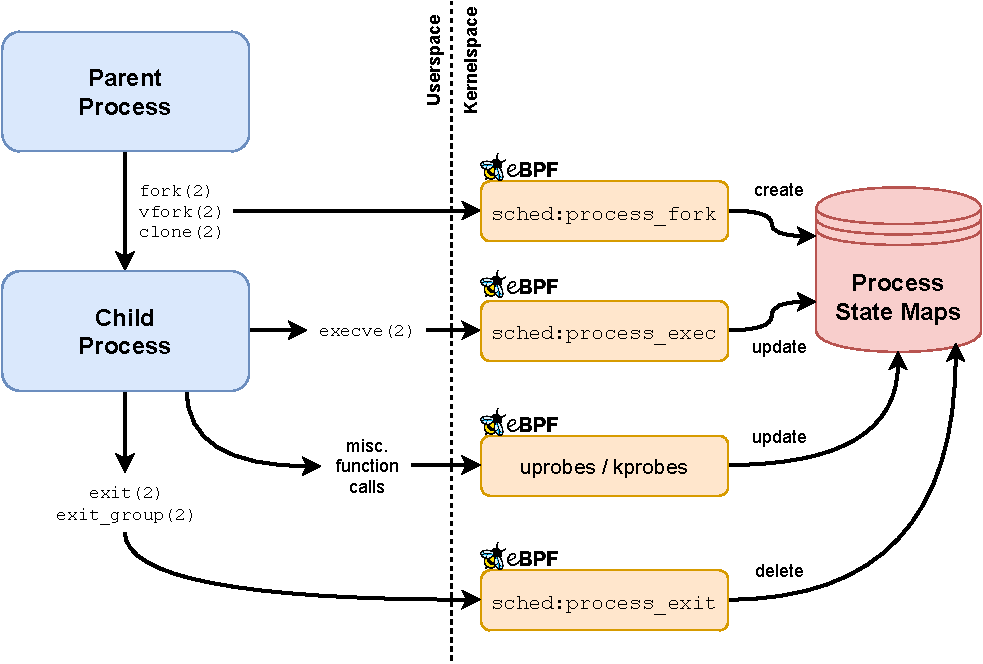
\includegraphics[width=0.8\linewidth]{figs/bpfbox/process-lifecycle.pdf}
     \caption[The various mechanisms that \bpfbox{} uses to manage process state]{
       The various mechanisms that \bpfbox{} uses to manage process state.
       Probes marked \texttt{sched:*} are tracepoints instrumenting scheduler events
       in the kernel. Uprobes and kprobes instrument userspace
       and kernelspace function calls respectively.
     }%
     \label{fig:bpfbox-process-lifecycle}
 \end{figure}

%% \begin{lstlisting}[language=c, caption={The data structure stored in the \textit{process states} hashmap,
%% which \bpfbox{} uses to track the state of running tasks. The map is keyed by
%% thread ID.}, label={lst:process-state}]
%% struct bpfbox_process_t {
%%     /* Key of the profile associated with
%%      * this process. */
%%     u64 profile_key;
%%     /* A 64-bit vector representing
%%      * the current state of the process. */
%%     u64 state;
%% };
%% \end{lstlisting}

Instrumenting a tracepoint on \texttt{sched:process\_fork} allows \bpfbox{} to
detect when a new task is created via the \texttt{fork(2)}, \texttt{vfork(2)}, or
\texttt{clone(2)} system calls. This tracepoint creates an entry in the \textit{process
states} hashmap and initializes it according to the state of the parent process; if the
parent process is associated with a \bpfbox{} profile, its key is copied to the child
until such time as the child makes an \texttt{execve(2)} call.

The \texttt{sched:process\_exec} tracepoint is triggered whenever a task calls
\texttt{execve} to load a new program.  \bpfbox{} uses this tracepoint to manage the
association of \textit{policy keys} to a particular \textit{process state}.  \bpfbox{}
policy may optionally specify whether a transition from one profile to another may occur
in a given call to \texttt{execve}; this transition is disallowed by default.

Finally, the \texttt{sched:process\_exit} tracepoint allows \bpfbox{} to detect when
a task exits. This tracepoint deletes the corresponding entry in the \textit{process
states} map.

\subsubsection{Context-Aware Policy}
\label{sec:context-aware}

If the policy for a given executable defines specific function call contexts for
particular rules, \bpfbox{} instruments these function calls using uprobes (for userspace
functions) and kprobes (for kernelspace functions). Each instrumented function call is
associated with a unique bit in the process' \textit{state} bitmask.  A probe is triggered
on entry that causes \bpfbox{} to flip the corresponding bit to a \texttt{1}, and again on
return, flipping the corresponding bit back to a \texttt{0}.
\Cref{fig:bpfbox-function-calls} depicts how \bpfbox{} instruments userspace and
kernelspace function calls for policy enforcement.

 \begin{figure}[p]
     \centering
     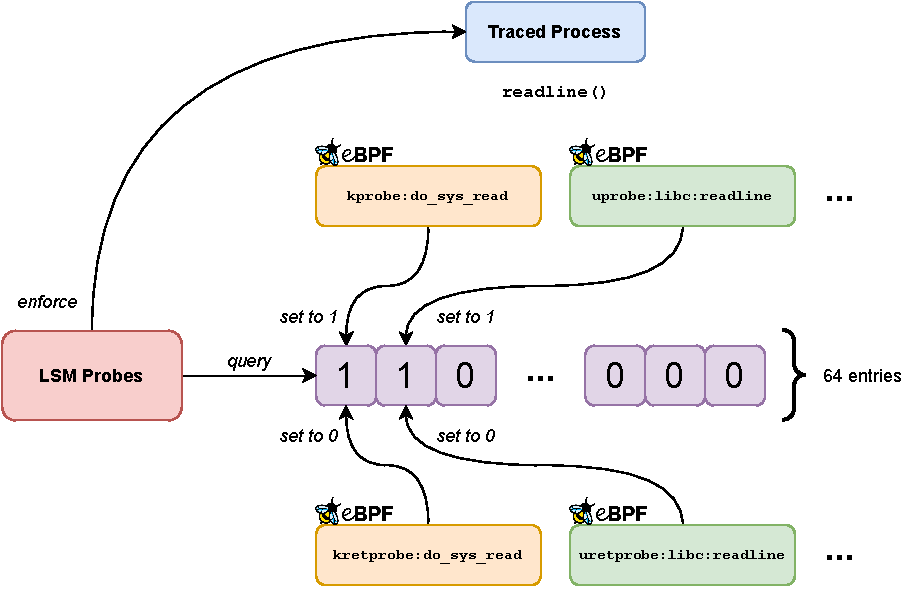
\includegraphics[width=1\linewidth]{figs/bpfbox/function-calls.pdf}
     \caption[How \bpfbox{} tracks function calls]{
       How \bpfbox{} uses kprobes and uprobes to track function calls.  If a policy
       identifies that a rule should apply within the context of a certain function call,
       \bpfbox{} instruments a probe on function entry and return. These probes flip the
       corresponding bit in the process' state vector, indicating to policy enforcement
       probes whether or not the process is in the middle of making the function call.
     }%
     \label{fig:bpfbox-function-calls}
 \end{figure}

This approach is subject to a few inherent limitations.  Firstly, compile-time
optimizations such as function in-lining can invalidate the probe by removing the
corresponding symbol in the target object file. Secondly, a recursive call that is not
tail-optimized will break enforcement by prematurely signalling to \bpfbox{} that
a process has exited a given function context.  The first limitation may be trivially
worked around by hinting to the compiler that a given function should not be in-lined;
although this sacrifices some application transparency and incurs a slight performance
penalty, the potential security benefits from such a fine-grained policy are arguably
worth the trade-off.  The second limitation \textit{could} be worked around by maintaining
a reference counter for each function call rather than a flat vector. \bpfbox{} currently
does not do this, since it would incur a larger memory overhead for each active process,
but it would be possible to extend a future version of \bpfbox{} with this workaround. In
case working around these limitations is impractical, the policy author would simply fall
back to specifying ordinary rules rather than context-specific ones.



\subsection{Collecting and Logging Audit Data}%
\label{ss:bpfbox-audit}

When an operation is denied or matches with an audit rule, \bpfbox{} submits an event to
userspace for logging. To accomplish this, we leverage the new ringbuf map type added in
Linux 5.8. The \gls{ebpf} ringbuf map implements an efficient ring buffer that is shared
across all \glspl{cpu}. This new map type comes with a number of optimizations for fast
reads and writes and in-order guarantees for asynchronous events across multiple
\glspl{cpu}, allowing per-event data to be efficiently shared with userspace in near
real-time.

In userspace, the \bpfbox{} daemon uses \texttt{mmap(2)} to map the corresponding memory
region and polls for new data at regular intervals. As events are consumed in userspace
they are removed from the ring buffer to make room for new events.  Since the ringbuf map
provides strong order guarantees and high performance under contention, we can ensure that
\bpfbox{} always provides highly reliable and performant per-event auditing.



\section{\bpfbox{} Policy Language}
\label{s:bpfbox-policies}

\todo{This section will present and document the policy language of \bpfbox{}, taken from our paper.}





\section{Limitations and the Transition Toward \bpfcontain{}}

\todo{This section will discuss limitations of \bpfbox{}, how it was a rough first-cut at
a solution to the confinement problem, and talk about the aspects of \bpfbox{} that
\bpfcontain{} improves upon.}

\begin{inprogress}
\begin{itemize}
  \item
\end{itemize}
\end{inprogress}
